% !TEX encoding = UTF-8 Unicode
% !TeX program = xelatex
% !TEX TS-program = XeLaTeX

\documentclass[12pt, a4paper]{article}
%\documentclass[12pt, a5paper]{article}
\usepackage{mathtools}
\usepackage{unicode-math}
\usepackage{comment}
\usepackage{wrapfig}
\usepackage{xfrac}
\usepackage{tikz}
\usetikzlibrary{arrows, decorations.markings}

\usepackage[pass]{geometry}
%\geometry{legalpaper, landscape, margin=1in}
\usepackage{fullpage}
\usepackage{setspace}
\usepackage[localise]{xepersian}
\setstretch{1.195}
\settextfont[Scale=1]{XB Niloofar}
\setlatintextfont[Scale=1]{XB Niloofar}%{Junicode} %Junicode
\setdigitfont{XB Niloofar}%{XB Zar}

\setlength{\parindent}{0ex}

\definecolor{answercolor}{HTML}{0080ff}
\newcommand{\vsp}{\vspace{34pt}}
\newcommand{\پاسخ}[2]{#1}
%\thispagestyle{empty}
%\newcommand{\پاسخ}[2]{\color{answercolor}\textbf{پاسخ: }#2\color{black}\vspace{-0.3cm}}

\begin{document}
		\tikzset{
		treenode/.style = {align=center, inner sep=0pt, text centered,
			font=\sffamily},
		arn_n/.style = {treenode, circle, white, font=\sffamily\bfseries, draw=black,
			fill=black, text width=1.5em},% arbre rouge noir, noeud noir
				normal/.style = {circle, white, font=\sffamily\bfseries, draw=black,
			fill=black, text width=1.5em},%
		arn_r/.style = {treenode, circle, red, draw=red, 
			text width=1.5em, very thick},% arbre rouge noir, noeud rouge
		arn_s/.style = {treenode, circle, black, draw=black, 
			text width=1.5em, very thick},% arbre rouge noir, noeud rouge
		arn_x/.style = {treenode, rectangle, draw=black,
			minimum width=0.5em, minimum height=0.5em, very thick}% arbre rouge noir, nil
	}
	\begin{tikzpicture}[remember picture,overlay]	\node[anchor=north,yshift=-1.5cm] at (current page.north) {\rl{به نام خدا}};
	\end{tikzpicture}%

\vspace{-1cm}
{\centering
	\textbf{کوئیز ششم درس ساختمان داده‌ها و الگوریتم‌ها}\\
مدرس: مهدی صفرنژاد       - ۴ خرداد ۹۸\\
\raggedleft\small
نام و نام خانوادگی: \\
}
\vspace{-0.5cm}
\پرش‌متوسط\پرخط‌ا\\
در سؤالاتی که توضیح خواسته شده، یک پاسخ کوتاه (حدوداً بین یک تا دو خط) مدنظر است. در سؤالاتی که خواستۀ مسئله توضیحی نیست، جواب نهایی کفایت می‌کند و نوشتن مراحل رسیدن به جواب نیاز نیست.\\

گراف وزن‌دار $G=(V,E)$ زیر داده شده است. توجه کنید مجموعۀ رأس‌ها $V=\{s, a, b, c\}$ و مجموعۀ یال‌ها $E=\{(s,a), (s,b), (a,b), (a,c), (b,c)\}$ است.

	\begin{center}
	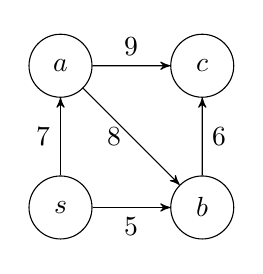
\begin{tikzpicture}[>=stealth', scale=1.8, auto,swap]
    \node[shape=circle,draw=black,minimum size=0.8cm] (s) at (0,0) {$s$};
    \node[shape=circle,draw=black,minimum size=0.8cm] (a) at (0,1) {$a$};
    \node[shape=circle,draw=black,minimum size=0.8cm] (b) at (1,0) {$b$};
    \node[shape=circle,draw=black,minimum size=0.8cm] (c) at (1,1) {$c$};
    
    \path [->] (s) edge node[left] {$7$} (a);
    \path [->] (s) edge node[below] {$5$} (b);
    \path [->] (a) edge node[left] {$8$} (b);
    \path [->] (a) edge node[above] {$9$} (c);
    \path [->] (b) edge node[right] {$6$} (c);
	\end{tikzpicture}
\end{center}
در این گراف می‌خواهیم کوتاهترین مسیر از رأس $s$ به بقیۀ را پیدا کنیم.
الگوریتم‌هایی که برای این کار مطرح کردیم، همه بر اساس اجرای تابع \متن‌لاتین{\متن‌تایپ{relax($u$,$v$)}} روی یال‌های مختلف بودند که هر الگوریتم این کار را با ترتیب خاصی انجام می‌داد. توجه کنید الگوریتم‌ها ممکن بود یک یال را چند بار relax کنند و هر بار فراخوانی این تابع لزوماً به تغییر $d[v]$ منجر نمی‌شود.

\پاراگراف{سؤال ۱.}
اگر الگوریتم کوتاهترین مسیر در DAG را روی گراف $G$ اجرا کنیم، تابع relax به چه ترتیبی روی یال‌ها صدا زده می‌شود؟

\پاسخ{\vsp\vsp}{
ترتیب یال‌ها در زیر آمده است. توجه کنید یال‌هایی که در $\{\}$ قرار گرفتند، ترتیب‌شان نسبت هم مهم نیست.
\begin{center}
$\{(s,a),(s,b)\},\{(a,b),(a,c)\},(b,c)$
\end{center}

}

\پاراگراف{سؤال ۲.}
اگر الگوریتم دکسترا (دایسترا) را روی گراف $G$ اجرا کنیم، تابع relax به چه ترتیبی روی یال‌ها صدا زده می‌شود؟


\پاسخ{\vsp\vsp}{
\begin{center}
$\{(s,a),(s,b)\},(b,c),\{(a,b),(a,c)\}$
\end{center}

}

\پاراگراف{سؤال ۳.}
اگر الگوریتم بلمن-فورد را روی گراف $G$ اجرا کنیم، تابع relax به چه ترتیبی روی یال‌ها صدا زده می‌شود؟

\پاسخ{\vsp\vsp}{
\begin{center}
$\{(s, a), (s,b), (b,c), (a,b), (a,c)\},$\\
$\{(s, a), (s,b), (b,c), (a,b), (a,c)\},$\\
$\{(s, a), (s,b), (b,c), (a,b), (a,c)\}$
\end{center}

}
	
\پاراگراف{سؤال ۴.}
گراف وزن‌داری داریم که وزن یال‌ها علاوه بر اعداد صحیح مثبت می‌تواند صفر، منفی یک و یا منفی دو باشد. آیا می‌توان به وزن همۀ یال‌ها ۳ واحد اضافه کرد و با اجرای الگوریتم دکسترا کوتاهترین مسیرها از رأس مشخص $s$ به بقیه را پیدا کرد؟

\پاسخ{\vsp\vsp}{
	خیر. گراف سه رأسی مسیر $P_3$ و رأس $t$ را به عنوان یک مقصد در نظر بگیرید. اگر برای وزن یال‌ها داشته باشیم $w(s,t)=-1$، $w(s,v)=0$ و $w(v,t)=-2$، در این صورت مسیر به درستی پیدا نمی‌شود.
	
}

\پاراگراف{سؤال ۵.}
آیا در درخت DFS یک گراف بدون جهت، طولانی‌ترین مسیر از مبدأ $s$ نیز وجود خواهد داشت؟

\پاسخ{\vsp\vsp}{
خیر. مثال نقض به سادگی پیدا می‌شود. توجه کنید DFS ممکن است همسایه‌ها را به ترتیب بدی پیمایش کند.
	
}

\پاراگراف{سؤال ۶. (۳ نمره)}
الگوریتمی برای پیدا کردن یک مسیر هامیلتونی (مسیری که از همۀ رأس‌های گراف عبور کند) در یک DAG (در صورت وجود) پیشنهاد دهید. مراحل الگوریتم را بگویید و زمان اجرا را نیز بیان کنید (اثبات نیاز نیست).

\پاسخ{\vsp\vsp\vsp\vsp}{
اگر یک DAG مسیر هامیلتونی داشته باشد، این مسیر مطابق با ترتیب توپولوژیک آن خواهد بود و ترتیب توپولوژیک هم در چنین گرافی یکتا است. بنابراین کافی است با یک DFS (به صورتی که در کلاس گفته شده) ترتیب توپولوژیک رأس‌های DAG را به‌دست آوریم و چک کنیم بین هر دو رأس متوالی یال جهت‌دار وجود داشته باشد. زمان اجرای این الگوریتم $O(n+e)$ خواهد بود.
	
}

\پاراگراف{سؤال ۷.}
آیا عمق درخت BFS برابر با قطر گراف است؟ (قطر گراف، بیشترین فاصله بین دو رأس گراف است. فاصله دو رأس کوتاهترین مسیر بین آن دو رأس است.)

\پاسخ{\vsp\vsp}{
خیر. در یک مسیر سه رأسی اگر از رأس وسط BFS اجرا شود، ارتفاع درخت ۱ است در صورتی که قطر گراف ۲ است.
	
}

\پاراگراف{سؤال ۸.}
آیا مسئلۀ تشخیص وجود یک زیرگراف کامل $k$ رأسی در یک گراف، یک مسئلۀ ان‌پی است؟

\پاسخ{\vsp\vsp}{
بله. زیرا در صورت داشتن $k$ رأس این زیرگراف به عنوان «اثبات»، می‌توانیم وجود همۀ یال‌های بین این $k$ رأس را در زمان چندجمله‌ای $O(k^2)=O(n^2)$ بررسی می‌کنیم.

به طور مشابه می‌توان گفت $k$ رأس را با سکه انداختن انتخاب می‌کنیم. سپس در زمان چندجمله‌ای 
	$O(k^2)=O(n^2)$ وجود همۀ یال‌های بین این $k$ رأس را بررسی می‌کنیم. 
	
این سؤال از مطالب جلسۀ آخر و خارج از مطالب درسی است.
	
}


\vspace{1pt}
\begin{flushleft}
موفق باشید
\end{flushleft}
\end{document}